\documentclass[12pt]{article} % Set base font size to 12pt
\usepackage{graphicx}
\usepackage{geometry} % Adjust page margins
\usepackage{setspace} % Line spacing
\usepackage{titlesec} % Customize section titles
\usepackage{tocloft} % Customize table of contents
\usepackage{fancyhdr} % Headers and footers
\usepackage{hyperref} % Add hyperlinks
\usepackage{xcolor} % Color package

% Set page margins
\geometry{a4paper, margin=2.5cm}

% Set line spacing
\setstretch{1.5} % Adjust line spacing for better readability

% Customize section titles
\titleformat{\section}[block]{\LARGE\bfseries\color{black}}{}{0em}{\filcenter}
\titlespacing*{\section}{0pt}{3.5ex plus 1ex minus .2ex}{2.3ex plus .2ex}

% Customize table of contents
\renewcommand{\cftsecleader}{\cftdotfill{\cftdotsep}}
\renewcommand{\contentsname}{Inhaltsverzeichnis}
\renewcommand{\cftaftertoctitle}{\par\nobreak\bigskip\bigskip\bigskip} % Add space after TOC title
\setlength{\cftbeforesecskip}{0.5em} % Adjust spacing between section entries
\setlength{\cftaftertoctitleskip}{2cm} % Adjust spacing between TOC title and entries
\hypersetup{
    colorlinks=true,
    linkcolor=blue,
    filecolor=magenta,
    urlcolor=cyan,
}

% Define headers and footers
\pagestyle{fancy}
\fancyhf{} % Clear default headers and footers
\fancyhead[R]{\thepage} % Page number on right side of header
\fancyhead[L]{\nouppercase{\leftmark}} % Chapter title on left side of header
\renewcommand{\headrulewidth}{0pt} % Remove header line
\fancyfoot[C]{\thepage} % Page number in the center of footer
\renewcommand{\footrulewidth}{0pt} % Remove footer line

% Define light gray color
\definecolor{lightgray}{RGB}{240,240,240}

\begin{document}

% Title Page
\begin{titlepage}
    \centering
    \vspace*{3cm}
    {\Huge\bfseries\textcolor{blue}{\MakeUppercase{ Kampf um die Wahrheit }}\par} % Increased font size and colored title
    \vspace{0.5cm} % Adjust space between title and author
    {\Large\textit{ Maja Schmidt }\par} % Italic author name
    \vfill
    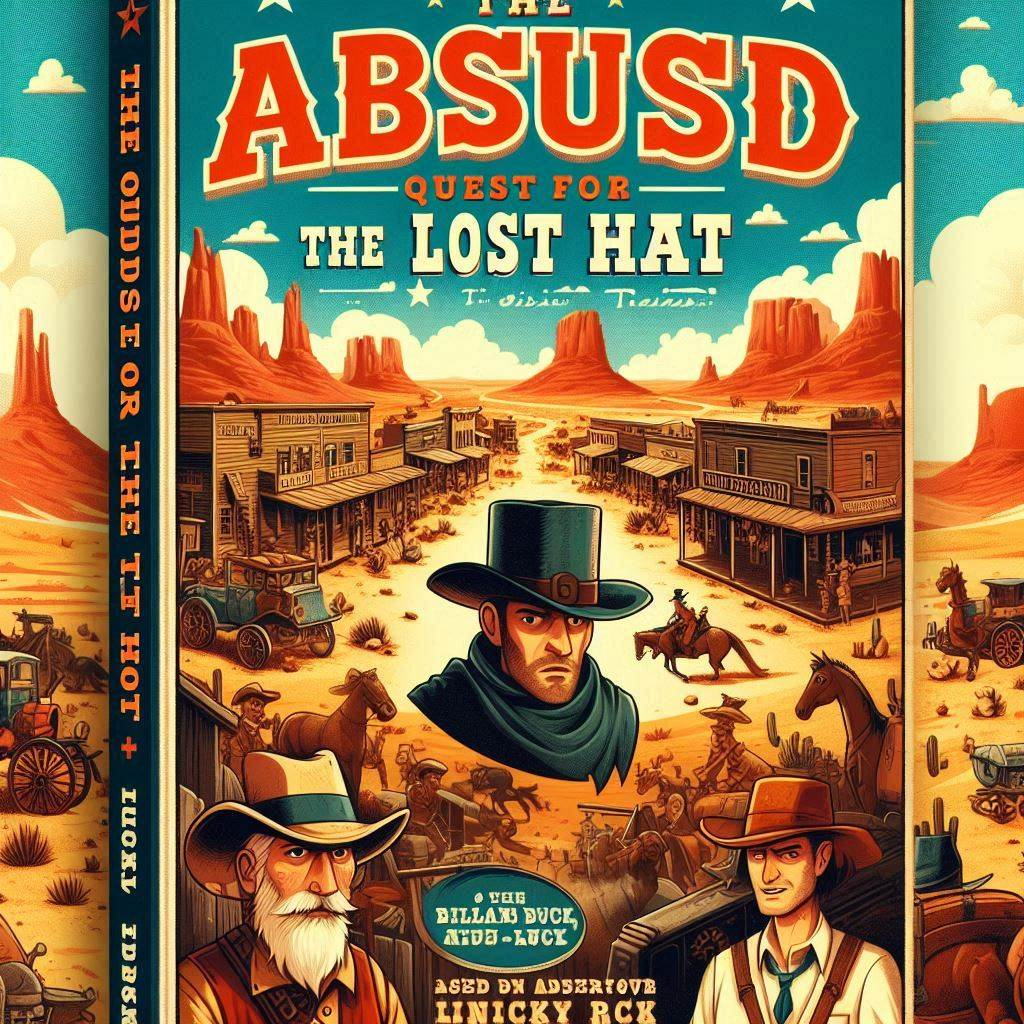
\includegraphics[width=0.9\textwidth]{ cover.jpg } % Larger cover image
    \vfill
    \today
\end{titlepage}

% Autorenvita
\section*{Autorenvita}
\vspace{4cm} % Adjust space between "Autorenvita" and "Inhaltsverzeichnis"
\begin{minipage}{\textwidth}
    Maja Schmidt ist eine renommierte Autorin von Fantasy-Romanen. Mit ihrer Fähigkeit, fesselnde Handlungen und komplexe Charaktere zu erschaffen, hat sie sich einen Namen in der Welt der Fantasy-Literatur gemacht. Ihre Werke zeichnen sich durch eine präzise und fokussierte Sprache aus, die es den Lesern ermöglicht, sich in die faszinierenden Welten und Charaktere einzufühlen.
\end{minipage}

% Place table of contents on a separate page
\clearpage
\tableofcontents
\clearpage

% Chapters

\section{ Die Entdeckung der verlorenen Magie }
\begin{minipage}{\textwidth}
    Elena spürte ein seltsames Kribbeln in ihren Fingerspitzen, als sie durch den verlassenen Wald streifte. Die Bäume schienen zu flüstern, und das Licht tanzte auf unerklärliche Weise um sie herum. Plötzlich entdeckte sie ein leuchtendes Symbol auf einem alten Baumstamm, das sie magisch anzog. Als sie es berührte, durchfuhr sie ein mächtiger Schauer und ein Strudel aus funkelnden Lichtern umhüllte sie. Verblüfft und verwirrt taumelte sie zurück und stieß gegen einen Fremden, der aus dem Nichts aufgetaucht zu sein schien. 'Du hast es gefunden', sagte er ruhig. 'Die verlorene Magie in dir.' Elena starrte ihn fassungslos an, unfähig zu begreifen, was gerade geschehen war. Der Fremde stellte sich als Kieran vor, ein erfahrener Wächter der verlorenen Magie. Er erklärte ihr die Bedeutung des Symbols und die Macht, die in ihr schlummerte. Von diesem Moment an wurde Elenas Welt auf den Kopf gestellt, und sie wurde in eine Welt voller Intrigen und Machtspiele eingeführt. Kieran versprach, sie in die Geheimnisse der verlorenen Magie einzuweihen und sie auf ihrem Weg zu unterstützen.
\end{minipage}

\section{ Intrigen am königlichen Hof }
\begin{minipage}{\textwidth}
    Elena fand sich inmitten der prächtigen Hallen des königlichen Hofes wieder, umgeben von funkelnden Kronleuchtern und kunstvollen Gemälden. Doch hinter der glanzvollen Fassade lauerten dunkle Intrigen und gefährliche Machtspiele. Sie spürte die Blicke der Höflinge auf sich ruhen, während sie versuchte, Lord Aric ausfindig zu machen. Plötzlich trat ein eleganter Mann mit durchdringendem Blick an sie heran. 'Eure Majestät, erlaubt mir, mich vorzustellen. Ich bin Lord Aric', sagte er mit einer verführerischen Stimme. Elena spürte eine unheimliche Kälte, als sie seinen Blick erwiderte. Sie wusste, dass er die verlorene Magie für seine eigenen finsteren Zwecke nutzen wollte. Inmitten der politischen Intrigen musste sie wachsam sein und herausfinden, wem sie vertrauen konnte. Plötzlich tauchte Kieran neben ihr auf, ein Schatten in der Menge. 'Sei vorsichtig, Elena. Nicht alles ist, wie es scheint', flüsterte er ihr zu. Gemeinsam versuchten sie, die Wahrheit aufzudecken und die verlorene Magie vor Missbrauch zu schützen. Doch die Gefahr lauerte an jeder Ecke, und Elena musste sich entscheiden, ob sie den Mut aufbringen konnte, sich den dunklen Mächten am königlichen Hof entgegenzustellen.
\end{minipage}

\section{ Der epische Kampf um die Zukunft der Magie }
\begin{minipage}{\textwidth}
    Die Nacht hüllte den königlichen Hof in ein düsteres Gewand, als Elena und Kieran sich auf den entscheidenden Kampf vorbereiteten. Die Sterne funkelten am Himmel, als ob sie die bevorstehende Schlacht beobachteten. Lord Aric hatte seine dunklen Kräfte mobilisiert und die verlorene Magie in einem verzweifelten Versuch, seine Macht zu festigen, entfesselt. Die Luft war erfüllt von der Spannung zwischen Gut und Böse, Hoffnung und Verzweiflung. Elena spürte die Energie in sich aufsteigen, während sie sich auf ihre Fähigkeiten und Stärken besann. Kieran stand an ihrer Seite, ein Symbol der Loyalität und Entschlossenheit. Gemeinsam traten sie Lord Aric entgegen, bereit, die Zukunft der Magie zu verteidigen. Der Kampf entbrannte in einem Wirbel aus magischen Strahlen und donnernden Elementen. Elena und Kieran kämpften mit vereinten Kräften, ihre Entschlossenheit und Mut waren unerschütterlich. Lord Aric, einst so manipulativ und machthungrig, sah sich nun einer unerbittlichen Konfrontation gegenüber. Die Wahrheit über die Vergangenheit und die Zukunft der Magie enthüllte sich inmitten des tobenden Gefechts. Elena erkannte, dass sie die Schlüsselrolle in diesem Kampf spielte, und sie schöpfte all ihre inneren Kräfte, um die verlorene Magie vor Missbrauch zu schützen. In einem atemberaubenden Moment der Erleuchtung entfalteten sich ihre Fähigkeiten zu ihrer vollen Pracht. Ein blendendes Licht umhüllte sie, und sie fühlte, wie die Magie in ihr und um sie herum erwachte. Mit einem kraftvollen Schlag des Lichts besiegte sie Lord Aric und bannte seine dunklen Machenschaften. Die verlorene Magie fand ihre wahre Bestimmung und kehrte in die Welt zurück, erneuert und gestärkt durch Elenas Mut und Opferbereitschaft. Die Sterne am Himmel schienen heller zu leuchten, als ob sie Elenas Sieg feierten. Kieran lächelte sie an, stolz und unterstützend. Die Zukunft der Magie war gerettet, und Elena hatte ihre wahre Größe und Stärke gefunden.
\end{minipage}

\clearpage
% Metadata
\section*{Metadaten}
\begin{minipage}{\textwidth}
    \colorbox{lightgray}{
        \begin{minipage}{\dimexpr\textwidth-2\fboxsep}
            \vspace{4cm}
            \begin{itemize}
                \item Name des Buches: Kampf um die Wahrheit
                \item Name des Autors: Maja Schmidt
                \item Name des Herausgebers: Mark Zimmermann
                \item Name des Verlags: HdM AI Technologies
                \item Adresse des Verlags: Nobelstraße 10, 70569 Stuttgart
                \item Datum der Veröffentlichung: 2022-10-20
            \end{itemize}
            \vspace{4cm}
        \end{minipage}

    }
\end{minipage}


\end{document}